%tp1_result.tex

\section{R\'esultats}

\subsection{Débits moyens}
La première étape consistait à déterminer les débits moyens respectifs des quatre liens.
Ainsi nous avons obtenu les résultats suivants :
\begin{itemize}
	\item UDP : 121545 octets/s = 950 kb/s
	\item TCP 1 : 112032 octets/s = 875 kb/s
	\item TCP 2 : 10917 octets/s = 85 kb/s
	\item TCP 3 : 7426 octets/s = 58 kb/s
\end{itemize}

Nous remarquons bien que les débits sont décroissants, ce qui est bien le résultat
attendu : en effet, l'UDP envoie sans attendre de réponse, tandis que les trois TCP sont
ordonnés par temps de latence croissant.
De plus, il est visible que les deux premiers liens utilisent presque toute la bande passante
disponible.

\subsection{Taux de perte}
La deuxième étape était de mesurer les taux de perte respectifs de chacun des liens.
Nous avons procédé de deux manières différentes, la première valeur est le taux de pertes
de paquets, tandis que la seconde est le taux de pertes en quantité d'information
(octets).
\begin{itemize}
	\item UDP : 3.58\% ; 3.58\% (taille de paquets fixée)
	\item TCP1 : 1.86\% ; 3.52\%
	\item TCP2 : 3.34\% ; 6.31\%
	\item TCP3 : 2.12\% ; 4.07\%
\end{itemize}
Le calcul des taux de pertes revient à diviser le nombre de paquets (resp. leur taille)
perdus par le nombre envoyé.
On remarque que les taux de perte ne sont pas si élevés du fait que les agents TCP
attendent une réponse avant de recommencer à envoyer.

\subsection{Taille de la file d'attente}

Comme nous pouvons le constater sur la figure suivante \ref{fa}, la taille de la file d'attente du lien augmente puis diminue
le temps que les messages soient traités.

\begin{figure}[!h]\label{fa}
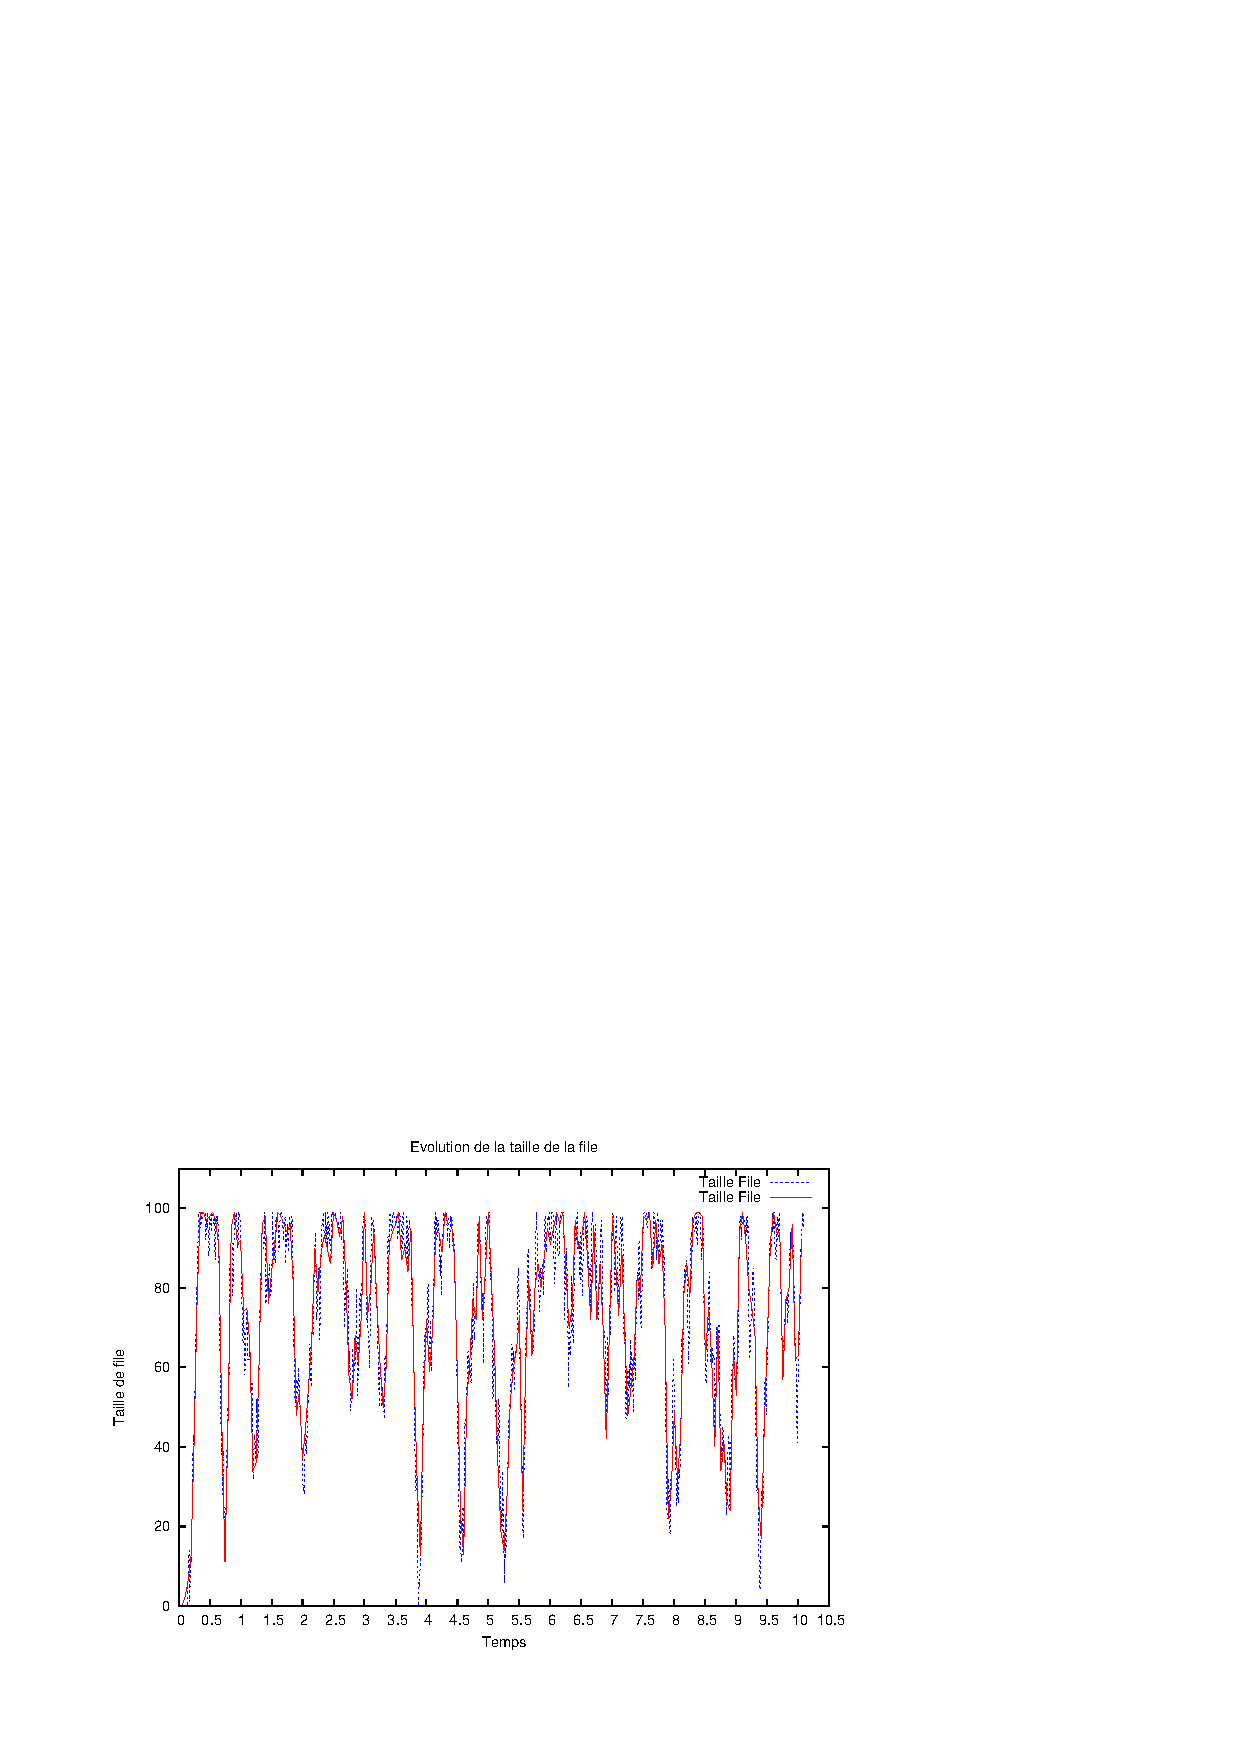
\includegraphics[scale=0.7]{../res/queuesize.png}
\caption{Evolution de la taille de la file d'attente au cours du temps}
\end{figure}

\subsection{Taille de la fenêtre TCP}

Sur la figure suivante \ref{fe} où les tailles des différentes fenêtres TCP sont représentées, nous observons que la première
connexion TCP utilise la majorité de la bande passante restante après le passage du trafic UDP. Ainsi les deux dernières
connexions ont une fenêtre qui diminue peu (étant donné que la fenêtre est réinitialisée à la réception d'un accusé et que ceux-ci ne peuvent pas circuler sur le lien surchargé).

\begin{figure}[!h]\label{fe}
\includegraphics[scale=0.7]{../res/winsize.png}
\caption{Evolution de la taille de la fenêtre TCP}
\end{figure}

